\documentclass[12pt]{article} 
\usepackage[utf8]{inputenc}
\usepackage{amsfonts}
\usepackage{algorithm}
\usepackage{fullpage}
\usepackage{enumitem}
\usepackage{graphicx}
\usepackage{amssymb}
\usepackage[utf8]{inputenc}
\usepackage{algorithmicx}
\usepackage{algpseudocode}
\usepackage{amsmath}
\usepackage{url}
\graphicspath{ {./images/} }

\title{ \centering Software Engineering Process - SOEN 6011 \\ Project Report}

\author{Saswati Chowdhury \\ ID : 40184906}

\date{5th August 2022}

\begin{document}

\maketitle
\noindent
\newpage
\noindent
\Large\textbf{Problem-1}
\section*{1.1 Introduction}


The tangent(tan) function, one of the primary six trigonometric functions, is typically expressed as $tan(x)$\textbf{\cite{cuemath_link}}.
\newline
The function as a ratio of the sine function to the cosine function, which can be obtained using a unit circle, is one way to define the tangent function\textbf{\cite{cuemath_link}}. The equation is as follows:
\newline
\newline
$tan(\theta) = \frac{ sin(\theta)}{cos(\theta) }$
\newline
\newline
It is the also the ratio of the angle's opposite and adjacent sides when a right-angled triangle is being considered\textbf{\cite{mathlearning_link}}. This can be referred to as:  
\newline
\newline
$tan( \theta ) = \frac{Opposite Side}{Adjacent Side}$
\newline
\section*{Characteristics\cite{cuemath_link}\cite{mathlearning_link}\cite{cuemath_domain}\cite{rapidtables_link}}
    \begin{itemize}
        \item Since tangent has the form $f(-x) = -f(x)$, it can be regarded as an odd function \textbf{\cite{cuemath_evenorodd}}.
        \item The tangent function is undefinable when $x = \pi / 2 + n \pi$ for which, cos(x) = 0 (where, n is integer)
        \item An intersecting line appears in both x and y axes at (0, 0)
        \item tan(x) is symmetric in nature.
        \item Period : $\pi $
        \item Below is a graph of the tangent function tan(x) \textbf{\cite{pic_link}}: 
        \begin{figure}[h!]
        \centering
            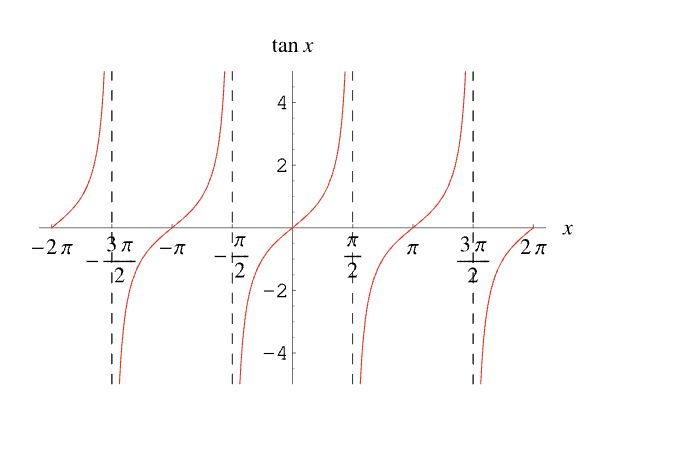
\includegraphics[width=12cm]{SEP1.png}
                \caption{ Graph of tangent function - $tan(x)$}
        \end{figure}
    \end{itemize}
    \pagebreak 
    
    
\section*{Domain and Co-Domain\cite{cuemath_domain}}
   \indent There are no values where cos x equals 0 in the $tan(x)$ domain. Hence, since $cos(x)$ is 0 at odd multiples of $\pi $/2, the domain and Co-Domain of tangent function can be expressed as follows: .
\begin{enumerate}
\item Domain : $ \{x\mid x \neq \frac{\pi}{2} + k\pi , k= ...,-1,0,1,...   \}$
\item Co-Domain : R
\end{enumerate}

\section*{1.2 Context of Use Model for the Tangent Calculator}
\begin{figure}[h!]
\centering
            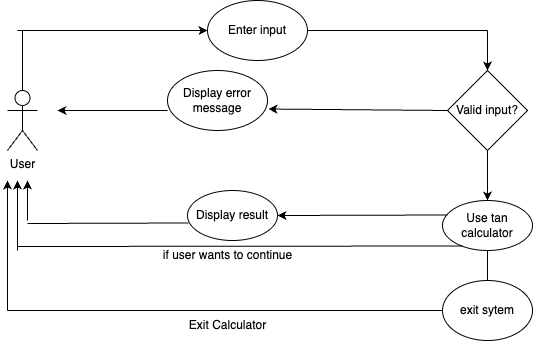
\includegraphics[width=10cm]{context.png}
                \caption{Context of Use Model}
        \end{figure}
    
\newpage
\noindent
\Large\textbf{Problem-2}
\section*{2.1 Functional Requirements}
\begin{enumerate}
        \item \textbf{First Requirement}
        \begin{itemize}
            \item \textbf{Label = } FR1
            \item\textbf{Difficulty = } Easy
            \item\textbf{Description = } The function $tan(x)$ allows the user to enter any valid number. For all the inputs, the $tan(x)$ function always provide valid values except for 
            $x = 2\pi + k\pi$. In this circumstance, $NaN$ may be returned.
        \end{itemize}

\item \textbf{Second Requirement}
        \begin{itemize}
            \item \textbf{Label = } FR2
            \item\textbf{Difficulty = } Easy
            \item\textbf{Description = } When $ x = \frac{\pi}{2} + k\pi$, $tan(x)$ returns $NaN$. $tan(x)$ does not satisfy the domain. The function gives back $NaN$. There is no need for calculation.
        
        \end{itemize}
        \item \textbf{Third Requirement}
        \begin{itemize}
            \item \textbf{Label = } FR3
            \item\textbf{Difficulty = } Easy
            \item\textbf{Description = } There is an incorrect format exception thrown when the input is non-numeric. Only numerical values can be passed to $tan(x)$. 
        \end{itemize}
        
        
        \item \textbf{Fourth Requirement}
        \begin{itemize}
            \item \textbf{Label = } FR4
            \item\textbf{Difficulty = } Medium
            \item\textbf{Description = } When $ x \neq \frac{\pi}{2} + k\pi$, $tan(x)$ returns the calculated value. As a result, the computed value will be returned.
        \end{itemize}
    \end{enumerate}
\section*{2.2 Assumptions}
    \begin{enumerate}
        \item Mathematically, the domain of a tangent function can be defined as a set of all possible real numbers. Hence, a real number needs to be entered as input.
        \item Based on the JAVA programming language, we assume the inputs fall within the acceptable numerical range. The range of user input should be between - 1.79769313486231570E+308 and + 1.79769313486231570E+308, depending on the data type chosen.
        \item In order to comply with the restrictions imposed by the programming language, only 16 decimal places are taken into account and those beyond 16 are removed automatically.
        \item For the purpose of the project, the value of pi is assumed to be 3.14159265358979323846 \textbf{\cite{wiki_pi}}.
        \item Due to the restrictions imposed on data types by programming languages, output values are also removed after 16 decimal digits.
    \end{enumerate}

\newpage
\noindent
\Large\textbf{Problem-3}
\section*{3.1 Mind Map Tangent Calculator}
\begin{figure}[h!]
\centering
\centering
    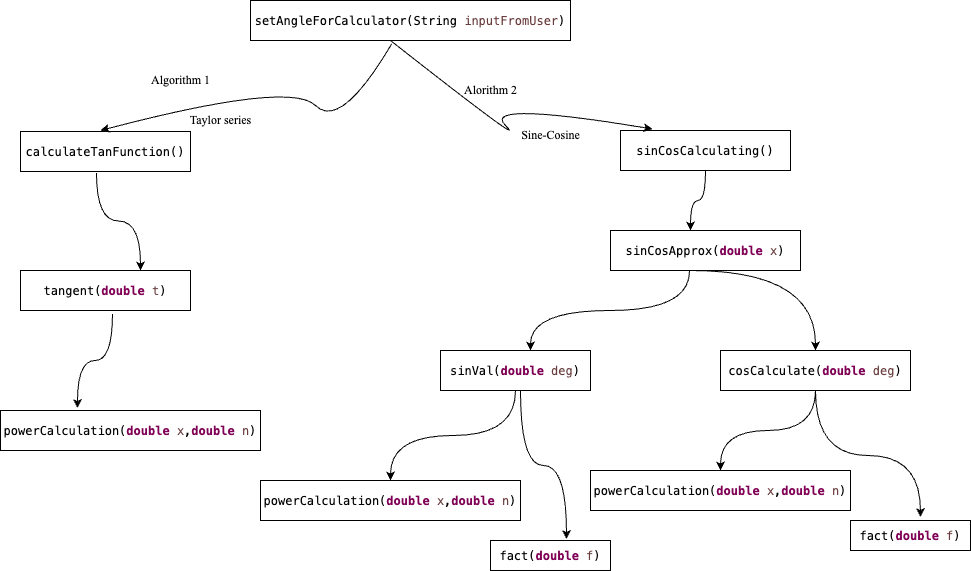
\includegraphics[scale=0.5]{mindmap.png}
    \caption{Mind map for Pseudocode Format}
\end{figure}

\section*{3.2 Algorithm-1 \cite{wiki_taylor}\cite{allmath_taylor}\cite{vedantu_taylor}\cite{quora_taylor}}
In a Taylor series, all differentials of a function f(x) are present in the region of a point as long as the function is continuous and all its differentials are present. In order to make a series of derivatives from the function, we need to know its order. 
It is represented as :\\~\\ 
% \[{F(x)} = \sum\propto n=0(f^{n}(a)n!(x-a)n)\]
$\sum_{n=0}^{\infty}\frac{f^{n}(a)}{n!}(x-a)^{n}$\
\newline
where,\
\newline
$f^{n}(a)$ is the function's nth order
\newline
The total number is $n$
\newline
The function's focal point is $a$
\newline
\textbf{Advantages}
\begin{itemize}
    \item When $x>=0$, the algorithm is applied to all possible real numbers.
    \item If the functional values and derivatives are recognised at a single point, it is utilised to assess the value of an entire function at each point.
    \item With this approach, a lot of mathematical proofs are simplified, and the sum of partial series can be used to approximate the entire series, which lowers the complexity of the code.
\end{itemize}

\textbf{Disadvantages}
\begin{itemize}
    \item The time it takes is the only drawback. In most circumstances, the only situations in which you should ever make use of it are when you need to find an odd value of a certain function, identify patterns in a proof, or locate integrals that are impossible to solve in any other way.
\end{itemize}

\textbf{Reasons to select this Algorithm}
\begin{itemize}
    \item This algorithm is employed for the power flow analysis.
    \item This can be applied to various optimization strategies, which entails approximating our function as a succession of linear or quadratic forms and iterating on them in order to determine the ideal value.
    
\end{itemize}

\pagebreak
\noindent
\textbf{Pseudocode for Algorithm 1}
\section*{Calculation of tan(x) using Taylor series expansion}


\begin{enumerate}
    \item start
    \item \indent user input
    \item validation checking for all conditions
    \item if x is outside of the range(0,180) then,
    \item \hspace*{10mm} the largest multiple of 180 lower than x is subtracted 
    \item end if
    \item if $ x$ is between $(90, 180)$ then,
    \item \hspace*{10mm} $ x  \leftarrow x - 180 $
    \item end if
    \item if $ x $ is between $(45, 90)$ then,
    \item \hspace*{10mm} $x1 \leftarrow 90 - x $
    \item \hspace*{10mm} return $ \frac{1}{ tan(x1) }  $
    \item end if
    \item if $ x $ is between $(22.5, 45)$ then,
    \item \hspace{10mm} return $ \frac{ 2*tan(\frac{x}{2})}{1 - tan^2(\frac{x}{2})}$
    \item end if 
    \item if $ x < 22.5 $ then,
    \item \hspace{10mm} $ z \leftarrow x * \frac{\pi}{180} $
    \item \hspace{10mm} return $ z + \frac{z^3}{3} + \frac{2z^5}{15} + \frac{17z^7}{315} $
\end{enumerate}
\newpage

\section*{3.3 Algorithm-2 \cite{baeldung_sincos}\cite{hindawi_link}}
The population-based metaheuristic technique known as the sine-cosine algorithm is used to solve optimization issues. Individuals within the population move within the search space to approximate the problem, which is done by optimizing. In order to do this, this algorithm utilizes trigonometric sine and cosine functions.
\newline


\textbf{Advantages}
\begin{itemize}
    \item Guarantee population diversity
    \item Enhance search capabilities
    \item Increasing the algorithm's performance, particularly when handling challenging optimization tasks
\end{itemize}

\textbf{Disadvantages}
\begin{itemize}
    \item The ratio of two independently obtained values are approximates, which is why this algorithm lacks accuracy.
    \item The calculation of sin(x) and cos(x) functions are necessary for this approach. Hence, takes longer to code and run.
\end{itemize}

\textbf{Reasons to select this Algorithm}
\begin{itemize}
    \item Any programming language may easily implement it.
    \item It saves time by quickly solving optimization issues.
\end{itemize}

\section*{Pseudocode for Algorithm 2}
\section*{Computing tan(x) as a ratio of sin and cos}

\begin{enumerate}
    \item start
    \item \indent user input
    \item validation checking
    \item if valid, 
    \Comment{\textbf{For $sin(x)$}},
    \item \hspace{10mm}$x1 \leftarrow sin(x)$\Comment{$sin(x)$ is calculated using Taylor's series}
    \item else
    \item \hspace{10mm} exit
    \item if valid, 
    \Comment{\textbf{for $cos(x)$}},
    \item \hspace{10mm} $x2 \leftarrow cos(x)$\Comment{$cos(x)$ is calculated using Taylor's series approximation}
    \item else
    \item \hspace{10mm} exit
    \item \textbf{For Sine-Cosine},
    \item if x == 90,
    \item \hspace{10mm} return NaN
    \item else
    \item \hspace{10mm} return $ \frac{x1}{x2}$\Comment{Final tan(x) value}
\end{enumerate}


\newpage
\noindent
\Large\textbf{Problem-4}
\section*{4.1 Programming Style \cite{monash_link}\cite{medium_link}}
Writing source code for a computer program requires adherence to a set of rules or guidelines, which are contained in a written document known as a programming style. A plugin \textbf{"google-java-format"} on IntelliJ version 2021 is available which is used in this program.\\
It helps programmers comprehend and maintain the code more easily and lowers the likelihood that they will make mistakes. Following a style guide eliminates unnecessary uncertainty and speculation.
\begin{figure}[h!]
\centering
            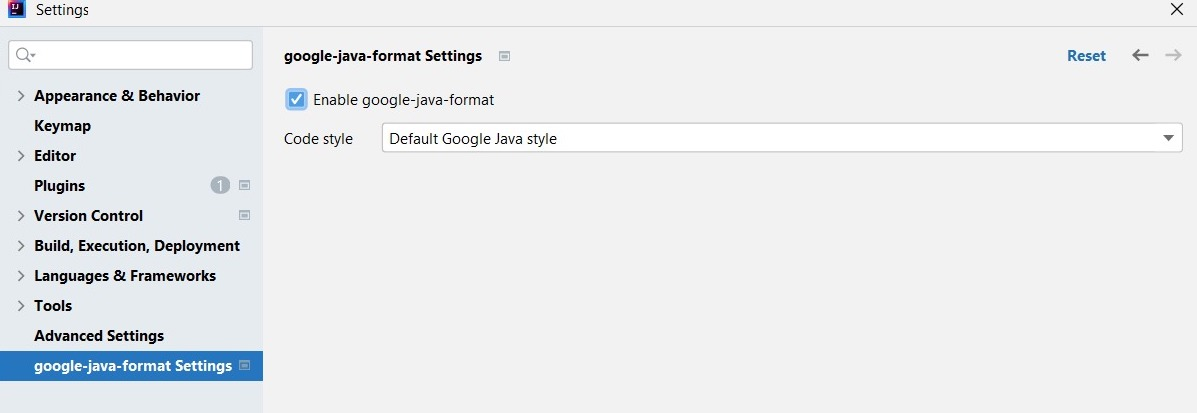
\includegraphics[width=12cm]{prog_style.png}
                \caption{Java Standard Programming Style}
        \end{figure}

\pagebreak
\section*{4.2 Error handling}
Errors occur as a result of improper operations carried out by a user \textbf{\cite{error_link}}. In order to continue maintaining the code, Java's exception handling mechanism is to ensure that programs run properly even after an exception is encountered and also provides security against system attacks\textbf{\cite{errorst_link}}.
In this program, there are try-catch blocks that are used to handle exceptions resulting from wrong input and other unforeseen circumstances.
\newline
\begin{figure}[h!]
\centering
            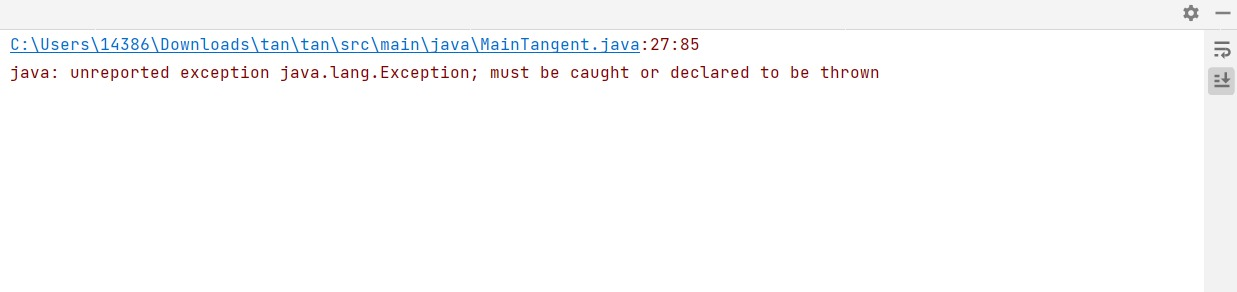
\includegraphics[width=12cm]{exception.png}
                \caption{Error Handling for Exception}
        \end{figure}


\section*{4.3 Debugger \cite{techopedia_link}\cite{javatpoint_link}\cite{jetbrains_link}\cite{gceasy_link}}
During the development of a program, programmers use a debugger to test the code in order to ensure that it is not behaving erratically. 
For implementing my assigned function tan(x), I am using the \textbf{Intellij IDE} and the \textbf{Intellij Debugger}.
\pagebreak
\section*{Advantages of Intellij Debugger}
    \begin{itemize}
        \item Implement specific breakpoints to inspect the state of the code and determine the value of expressions based on their analysis
        \item Sessions for debugging can be paused and resumed
        \item Errors can easily be detected and Memory usage analysis
    \end{itemize}


\section*{Disadvantages of Intellij Debugger}
    \begin{itemize}
        \item It consumes more system RAM and needs to have a high-end setup in order to run the InteliJ debugger.
        \item As part of the Intellij IDE for Java, Intellij Debugger is not convenient to use alone.
    \end{itemize}
    
    \begin{figure}
    \centering
            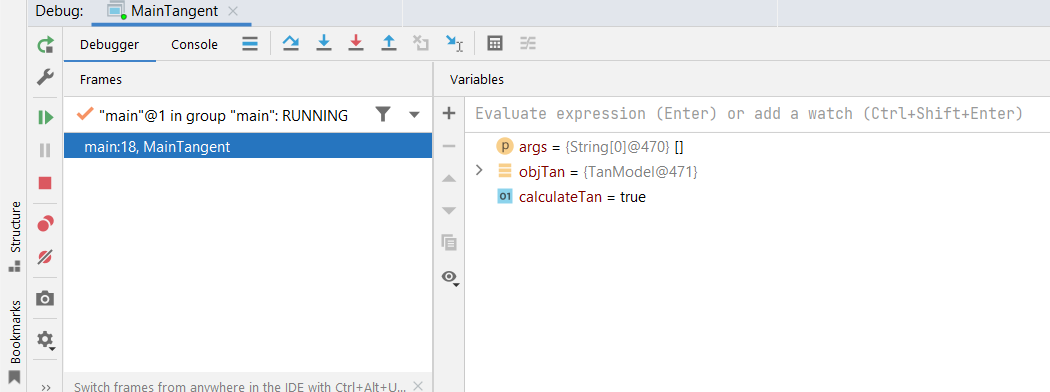
\includegraphics[width=12cm]{debug.png}
                \caption{: Debugging the main function}
        \end{figure}

\section*{4.4 Quality Criterion}
    \begin{enumerate}
        \item \textbf{Space Efficient}
        \newline
        During the development of this program, the creation variables were reduced in order to make the program space-efficient. There were not nested loops included in the program to save the space. Google programming style helps in removing unnecessary blank spaces.
        \item \textbf{Portable}
        \newline
        This program is platform independent. Without any installer, it runs perfectly.
        \item \textbf{Maintainable}
        \newline
        Modularizing the main functionality, handling errors, and user interactions have been done correctly. This facilitates updating of the code and the inclusion of new features easily. The appropriate details are added as comments for better understanding.
        \item \textbf{Correct}
        \newline
        To ensure that the program is correct, output is compared to values that have already been computed. Test cases based on Junit are used to ensure accuracy of the implemented application.
        \item \textbf{Robust}
        \newline
        Validation is performed on user input to ensure that only numeric values are entered. Data type compatibility is verified beforehand the computation. If the output exceeds the data type's limit, display the appropriate error message to the user.
        \item \textbf{Time Efficient}
        \newline
        The software functions effectively as the output is shown in 87 milliseconds after running all the test cases.
        \pagebreak
        \begin{figure}[h!]
        \centering
            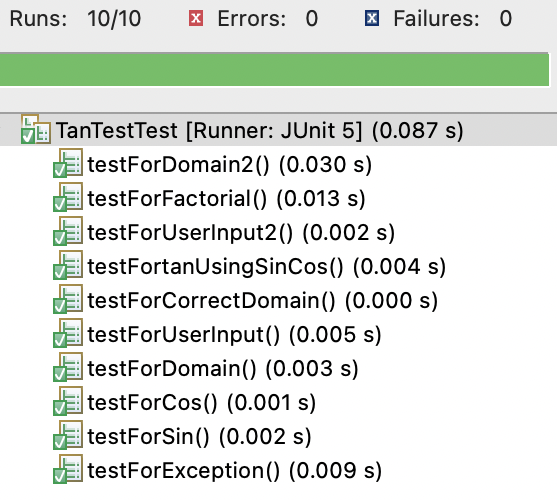
\includegraphics[scale=1.25]{test2.png}
                \caption{Showing Time for JUnit Test Cases}
        \end{figure}
        \item \textbf{Usable}
        \newline
        The user is presented with a text-based user interface that is incredibly straightforward and clear. In addition, the user can easily understand the results and error messages due to their clarity.
        
    \end{enumerate}


\section*{4.5 Checkstyle \cite{wiki_check}}
CheckStyle is a tool that examines the source code to see if it adheres to a specified coding style. The document's readability is  enhanced with the aid of this tool.
\section*{Advantages}
    \begin{itemize}
        \item Easily set up for continuous integration 
        \item operates effectively and enables the configuration of user-defined rules as well as making the code more understandable by examining for design and formatting flaws
    \end{itemize}
\section*{Disadvantages}
    \begin{itemize}
        \item Does not examine the code for any design flaws.
        \item It solely involves code beautifying; There are no logic checks.
    \end{itemize}
    
    \begin{figure}[h!]
    \centering
            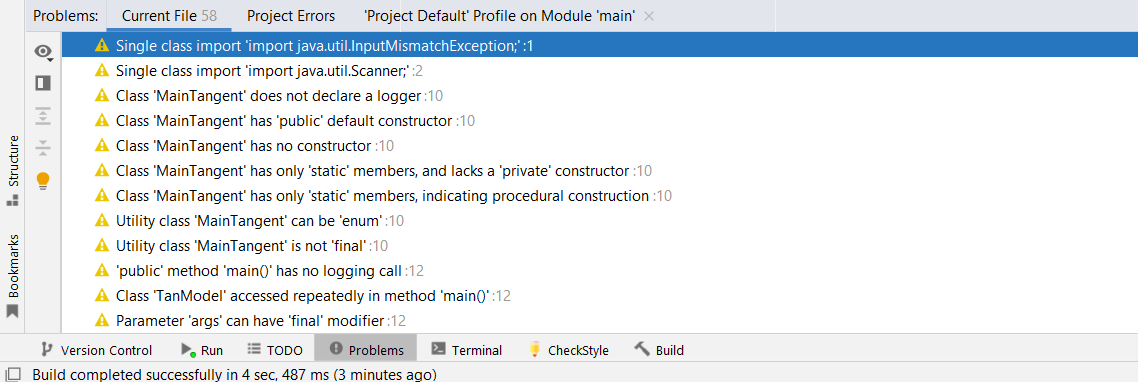
\includegraphics[scale=0.7]{checkstyle.png}
                \caption{Notification of check style suggestions}
        \end{figure}
\newpage
\noindent
\Large\textbf{Problem-5}
\section*{5.1 JUnit Standards}
In order to write and validated the unit tests of the given function, I used the JUnit framework. In all test cases, the functional requirements were met and the tests were conducted successfully.
\section*{5.2 Traceability to Requirements}
\begin{enumerate}
        \item FR1\\
        JUnit test cases: testForCorrectDomain()\\
        Description: By performing this test, it is confirmed that this function will produce the appropriate and correct value for the user who enters a valid angle.
        
        \item FR2\\
        JUnit test cases: testForDomain(), testForDomain2()\\
        Description: This test verifies that tan(x) returns NaN without computing it if the domain is not satisfied.
        
        \item FR3\\
        JUnit test cases: testForException()\\
        Description: This test verifies that an exception is raised for improper format if the input is not numeric.
        
        \item FR4\\
        JUnit test cases: testForUserInput(), testForUserInput2(),  testForFactorial(), testForSin(), testForCos(), testFortanUsingSinCos()\\
        Description: As a result of this test, it has been confirmed that tan(x) returns the computed value if domain is satisfied, including the correct value for it's subordinate function.

    \end{enumerate}

\begin{thebibliography}{9}
\bibitem{cuemath_link}
\url{https://www.cuemath.com/trigonometry/tangent-function/}
\bibitem{mathlearning_link}
\url{https://www.onlinemathlearning.com/tangent-function.html}
\bibitem{cuemath_evenorodd}
\url{https://www.cuemath.com/questions/is-tangent-even-or-odd/}
\bibitem{pic_link}
\url{https://mathworld.wolfram.com/Tangent.html}
\bibitem{cuemath_domain}
\url{https://www.cuemath.com/trigonometry/domain-and-range-of-trigonometric-functions/}
\bibitem{rapidtables_link}
\url{https://www.rapidtables.com/math/trigonometry/tan.html#rules}
\bibitem{wiki_pi}
\url{https://en.wikipedia.org/wiki/Pi}
\bibitem{wiki_taylor}
\url{https://en.wikipedia.org/wiki/Taylor_series}
\bibitem{allmath_taylor}
\url{https://www.allmath.com/taylor-series-calculator.php#what-is-the-taylor-series}
\bibitem{vedantu_taylor}
\url{https://www.vedantu.com/formula/taylor-series-formula}
\bibitem{quora_taylor}
\url{https://www.quora.com/What-are-the-advantages-and-disadvantages-of-the-Taylor-series-method}
\bibitem{baeldung_sincos}
\url{https://www.baeldung.com/cs/sine-cosine-algorithm}
\bibitem{hindawi_link}
\url{https://www.hindawi.com/journals/mpe/2020/8184254/}
\bibitem{monash_link}
\url{https://www.monash.edu/it/current-students/resources-and-support/style-guide/programming-styles}
\bibitem{medium_link}
\url{https://medium.com/level-up-web/what-is-a-programming-style-guide-and-why-should-you-care-9019e51bb7ad}
\bibitem{techopedia_link}
\url{https://www.techopedia.com/definition/597/debugger}
\bibitem{javatpoint_link}
\url{https://www.javatpoint.com/intellij-idea-debugging#:~:text=IntelliJ}
\bibitem{jetbrains_link}
\url{https://blog.jetbrains.com/idea/2020/05/debugger-basics-in-intellij-idea/}
\bibitem{gceasy_link}
\url{https://blog.gceasy.io/2018/11/05/memory-efficient-eclipse-or-intellij/}
\bibitem{error_link}
\url{https://www.geeksforgeeks.org/types-of-errors-in-java-with-examples/}
\bibitem{errorst_link}
\url{https://stackoverflow.com/questions/368139/why-is-error-handling-important}
\bibitem{wiki_check}
\url{https://en.wikipedia.org/wiki/Checkstyle}

\end{thebibliography}

    
    
\end{document}
